\documentclass[../../main.tex]{subfiles}

\begin{document}
\section{No Power-Law in Hidden Markov Models}
    When modelling \emph{natural language}, we generate the next token(s) based on the previous tokens (and hence not based on future tokens; we generate text from left to right). Thus, when disregarding the future tokens, i.e. when marginalizing over them, we can determine the Markov blanket of the current token, i.e. determine the minimal set of tokens that infuluence the current one.

    Naturally, we can think of natural language modelling as \emph{Bayesian networks} over the characters in the text. Because we generate text from left to right, we naturally assume all arrows to go from previous tokens to future tokens (because this is also the modus operandi for token generation). For example, Markov chains up to character position $t$ have the following simple representation:

    \begin{figure}[h]
        \center
        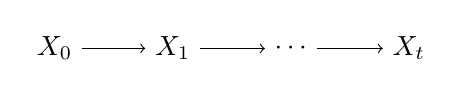
\begin{tikzpicture}[node distance=1.5cm, auto]
        \node (X0) {$X_0$};
        \node (X1) [right of=X0] {$X_1$};
        \node (dots) [right of=X1] {$\cdots$};
        \node (Xt) [right of=dots] {$X_t$};

        \draw[->] (X0) -- (X1);
        \draw[->] (X1) -- (dots);
        \draw[->] (dots) -- (Xt);
        \end{tikzpicture}
        \caption{Bayesian network of Markov chains. All arrows go from previous tokens to future tokens.}
        \label{fig:bayesian_network_markov_chain}
    \end{figure}

    But really, in Markov chains $P(X_{t + 1} = a \mid X_t = b)$ is independent of $t$ and hence is constant over time. So really, all the arrows in figure~\ref{fig:bayesian_network_markov_chain} represent the same transition, this is very important to note.

    From a modelling perspective, it is very reasonable to reuse the same transitions over time, as we cannot have infinitely many "hard-coded" transitions (but we can use different models whith implicitely infitite transitions). Furthermore, for the same \emph{mode of transition}, which we define as the "arrow structure" of all ingoing edges into the current node in the Bayesian network (in figure~\ref{fig:bayesian_network_markov_chain} the mode of transition would be from the current token to the next), it seems reasonable to assume invariance in time, i.e. fixed transition probabilities. We call such transitions to be \emph{constant}.

    Now, the question is, can we achieve power law decay with only one constant (hard-coded) mode of transition? Well, for Markov chains it did not work, so maybe we just have to augment the context window and create new modes of transition.

    This is an interesting approach, which we will investigate on. Since we already established interesting results for Markov chains, we would like to reduce any constant mode of transition to a Markov chain. But how do we do this for a larger context window, where we have many random variables influencing the current one?
    
    The idea is to employ a hidden variable $Y \in \Sigma ^s$, where $\Sigma$ is the alphabet, and $s$ is the size of the context window, which we define as the length of the longest arrow in the mode of transition (for Markov chains $s = 1$). Clearly, $Y$ captures the entire \emph{state} at time $t$ of our model, and we can model the transitions $Y_t \to Y_{t + 1}$ as simple Markov chain transitions (and hence independent of time). And, of course, once we know $Y_t$, we also know $X_t$ (which of course can be modelled with Markov chain transitions as well). Thus, we have the following Bayesian network:

    \begin{figure}[h]
        \center
        \begin{tikzpicture}[node distance=1.5cm and 1.5cm, auto]

        % Top row (Y)
        \node (Y0) {$Y_0$};
        \node (Y1) [right of=Y0] {$Y_1$};
        \node (Ydots) [right of=Y1] {$\cdots$};
        \node (Yt) [right of=Ydots] {$Y_t$};

        % Bottom row (X)
        \node (X0) [below of=Y0] {$X_0$};
        \node (X1) [right of=X0] {$X_1$};
        \node (Xdots) [right of=X1] {$\cdots$};
        \node (Xt) [right of=Xdots] {$X_t$};

        % Horizontal arrows (Y row)
        \draw[->] (Y0) -- (Y1);
        \draw[->] (Y1) -- (Ydots);
        \draw[->] (Ydots) -- (Yt);

        % Vertical arrows
        \draw[->] (Y0) -- (X0);
        \draw[->] (Y1) -- (X1);
        \draw[->] (Yt) -- (Xt);

        \end{tikzpicture}
        \caption{Bayesian network of a hidden Markov model.}
        \label{fig:bayesian_network_hidden_markov}
    \end{figure}

    \bigskip
    These models are known as \emph{hidden Markov models}. Unfortunately, there is no free lunch, as we will see in the following. But first, we will prove some lemmas.

    \begin{lemma}
        \label{lemma:raising_marov_matrix_to_its_period}
        Let $\bm{M}$ be the transition matrix for an irreducible Markov chain with period $p$. Then the chain described by $\bm{M}^p$ consists of exactly $p$ aperiodic, closed communication classes.
    \end{lemma}
    \vspace{-2.5em}
    \begin{proof}
        A key property of an irreducible Markov chain with period $p$ is that its state space $S$ can be uniquely partitioned into $p$ disjoint nonempty sets, called cyclic classes:
        \[
            S = C_0 \cup C_1 \cup \dots \cup C_{p-1} \quad .
        \]
        These classes are defined such that a one-step transition from any state in class $C_k$ can only lead to a state in the next class, $C_{(k+1) \pmod p}$.

        \textbf{Proving there are $p$ Closed Classes} \\
        Let's consider the chain governed by the transition matrix $\bm{M}^p$, which represents taking steps of size $p$. If we start in any state $s \in C_k$, after one step of the new chain (which is $p$ steps in the original chain), we will transition from $C_k \to C_{(k+1) \pmod p} \to \dots \to C_{(k+p) \pmod p}$.
        
        Since $(k+p) \pmod p = k$, any transition of length $p$ starting in $C_k$ must end in a state that is also in $C_k$. This means that for any state $s \in C_k$ and any state $t \notin C_k$, the transition probability is $(\bm{M}^p)_{st} = 0$.
        
        Since transitions under $\bm{M}^p$ from $C_k$ can only lead to states within $C_k$, each cyclic class is a closed communication class in the new chain. Furthermore, the partition gives us exactly $p$ such classes: Because the original chain is irreducible, every state must belong to one of these classes, and each class must be able to reach the next, ensuring all $p$ classes are part of the overall structure and are non-empty.

        \textbf{Proving Aperiodicity} \\
        Now we must show that each of these $p$ classes is aperiodic in the $\bm{M}^p$ chain. Based on lemma~\ref{lemma:return_states_with_period}, we know that for every state $i$ there exists an $\ell \in \mathbb{N}$ s.t. $\ell p$ and $(\ell + 1) p$ are both return times in $\bm{M}$. Hence, $\ell$ and $\ell + 1$ are return times in $\bm{M}^p$, and thus state $i$ is aperiodic in $\bm{M}^p$.
    \end{proof}

    \begin{lemma}
        \label{lemma:irreducible_aperiodic_markov_chain_stays_irreducible_aperiodic}
        Let $\bm{M}$ describe an irreducible aperiodic Markov chain. Then, for every $n \in \mathbb{N}_{>0}$, the Markov chain described by $\bm{M}^n$ is also irreducible and aperiodic.
    \end{lemma}
    \vspace{-2.5em}
    \begin{proof}
        Since $\bm{M}$ is irreducible and aperiodic, there exists an $m \in \mathbb{N}_{>0}$ s.t. $\bm{M}^m > \bm{0}$ based on theorem~\ref{theorem:positive_transition_matrix}. Hence, $\bm{0} < \bm{M}^{mn} = (\bm{M}^n)^m$. Finally, using corollary~\ref{corollary:converse_positive_transition_matrix}, it follows that $\bm{M}^n$ is irreducible and aperiodic.
    \end{proof}

    \begin{lemma}[Hidden Markov Models have the Bulk Marginal Property]
        Every hidden Markov model with finite state spaces $(S_Y, S_X)$ for its latent variable $Y$ and observable variable $X$ with transition matrices $(\bm{M_Y}, \bm{M_X})$ complies with the bulk marginal property.
    \end{lemma}
    \vspace{-2.5em}
    \begin{proof}
        Let $w_i \coloneqq X_{i - 1}$ for $n \in [n + 1]$. Then we have:
        \begin{align*}
            &\sum_{w_{n + 1} \in \Sigma} S_{n + 1}(w) \\
            &\underset{\text{Bayesian network}}{=} \sum_{w_{n + 1} \in \Sigma} \sum_{q_1, \dots, q_{n+1} \in S_Y} \left[ P(q_1) \prod_{i=2}^{n+1} P(q_i \mid q_{i-1}) \cdot \prod_{i=1}^{n+1} P(w_i \mid q_i) \right] \\
            &= \sum_{q_1, \dots, q_{n+1} \in S_Y} \sum_{w_{n + 1} \in \Sigma}  \left[ P(q_1) \prod_{i=2}^{n+1} P(q_i \mid q_{i-1}) \cdot \prod_{i=1}^{n+1} P(w_i \mid q_i) \right] \\
            &= \sum_{q_1, \dots, q_{n+1} \in S_Y} \left[ P(q_1) \prod_{i=2}^{n+1} P(q_i \mid q_{i-1}) \cdot \prod_{i=1}^{n} P(w_i \mid q_i) \sum_{w_{n + 1} \in \Sigma}  P(w_{n+1} \mid q_{n+1}) \right] \\
            &= \sum_{q_1, \dots, q_{n+1} \in S_Y} \left[ P(q_1) \prod_{i=2}^{n+1} P(q_i \mid q_{i-1}) \cdot \prod_{i=1}^{n} P(w_i \mid q_i) \right] \\
            &= \sum_{q_1, \dots, q_{n} \in S_Y} \sum_{q_{n+1} \in S_Y} P(q_{n+1} \mid q_n) \left[ P(q_1) \prod_{i=2}^{n} P(q_i \mid q_{i-1}) \cdot \prod_{i=1}^{n} P(w_i \mid q_i) \right] \\
            &= \sum_{q_1, \dots, q_{n} \in S_Y} \left[ P(q_1) \prod_{i=2}^{n} P(q_i \mid q_{i-1}) \cdot \prod_{i=1}^{n} P(w_i \mid q_i) \sum_{q_{n+1} \in S_Y} P(q_{n+1} \mid q_n) \right] \\
            &= \sum_{q_1, \dots, q_{n} \in S_Y} \left[ P(q_1) \prod_{i=2}^{n} P(q_i \mid q_{i-1}) \cdot \prod_{i=1}^{n} P(w_i \mid q_i) \right] \\
            &\overset{\checkmark}{=} S_n(w_{-\{n+1\}}) \quad .
        \end{align*}
    \end{proof}

    \begin{lemma}
        \label{lemma:exponential_convergence_with_open_states}
        Let
        \[
            \bm{M} \coloneqq
            \begin{bmatrix}
                \bm{A} & \bm{B} \\
                \bm{0} & \bm{C}
            \end{bmatrix}
        \]
        be a matrix consisting of submatrices \( \bm{A} \in \mathbb{R}^{k \times k} \), \( \bm{B} \in \mathbb{R}^{k \times \ell} \), and \( \bm{C} \in \mathbb{R}^{\ell \times \ell} \). Let $\bm{A}$ be an irreducible aperiodic Markov transition matrix, and let $\bm{C}^n \xrightarrow{n \to \infty} \bm{0}$ with exponential decay.
        Then, $\bm{M}^n$ decays exponentially in $n$ towards a matrix $\bm{M}'$.
    \end{lemma}
    \vspace{-2.5em}
    \begin{proof}
        Using induction, it is easy to show that
        \[
            \bm{M}^n =
            \begin{bmatrix}
            \bm{A}^n & \sum_{i=0}^{n-1} \bm{A}^{n-1-i} \bm{B} \bm{C}^i \\
            \bm{0} & \bm{C}^n
            \end{bmatrix}
            \quad .
        \]
        We aim to show that this sum converges to a finite matrix:
        \[
        \lim_{n \to \infty} \sum_{i=0}^{n-1} \bm{A}^{n-1-i} \bm{B} \bm{C}^i \eqqcolon \bm{D}_\infty \quad .
        \]
        Let us denote:
        \[
        \bm{D}_n := \sum_{i=0}^{n-1} \bm{A}^{n-1-i} \bm{B} \bm{C}^i \quad .
        \]
        We want to show that $\|\bm{D}_{n+1} - \bm{D}_{n}\| \leq c e^{-\alpha n}$ for some $\alpha \in \mathbb{R}_{> 0}$. Note that the exponentially fast convergence of $\bm{D}_{n}$ is equivalent to exponentially fast convergence of every entry in the matrix.
        
        Since $\bm{A}$ is irreducible and aperiodic, it follows that $\lambda_1 = 1$ and $|\lambda_2| < 1$ based on theorem~\ref{theorem:perron_frobenius}. Hence, it converges exponentially fast with a basis of $|\lambda_2|$.

        Furthermore, note that every entry $\alpha$ in every matrix for every $n$ is bounded by $\alpha \in [0, 1]$. Hence, we can argue about their element-wise deviation in big $\mathcal{O}$ notation where the hidden constants remain bounded:

        \begin{align*}
            &\bm{D}_{n+1} - \bm{D}_{n} \\
            &= \sum_{i=0}^{n} \bm{A}^{n-i}\bm{BC}^i - \sum_{i=0}^{n-1} \bm{A}^{n-1-i}\bm{BC}^i \\
            &= \bm{BC}^n + \sum_{i=0}^{n-1} \left[ \bm{A}^{n-i}\bm{BC}^i - \bm{A}^{n-1-i}\bm{BC}^i \right] \\
            &= \bm{BC}^n + \sum_{i=0}^{\frac{n}{2}-1} \left[ \left( \bm{A}^{n-i} - \bm{A}^{n-1-i} \right) \bm{BC}^i \right] + \sum_{\frac{n}{2}}^{n-1} \left[ \left( \bm{A}^{n-i} - \bm{A}^{n-1-i} \right) \bm{BC}^i \right] \\
            &= \pm \mathcal{O}(e^{-\alpha_1 n}) + \sum_{i=0}^{\frac{n}{2}-1} \left[ \left( \bm{A}^{n-i} - \bm{A}^{n-1-i} \right) \bm{BC}^i \right] + \sum_{\frac{n}{2}}^{n-1} \left[ \left( \bm{A}^{n-i} - \bm{A}^{n-1-i} \right) \bm{B} \cdot \mathcal{O}(e^{-\alpha_1 \frac{n}{2}}) \right] \\
            &= \pm \mathcal{O}(e^{-\alpha_1 n}) + \sum_{i=0}^{\frac{n}{2}-1} \left[ \left( \bm{A}^{n-i} - \bm{A}^{n-1-i} \right) \bm{BC}^i \right] \pm \mathcal{O}(n e^{-\alpha_1 \frac{n}{2}}) \\
            &= \pm \mathcal{O}(e^{-\alpha_1 n}) + \sum_{i=0}^{\frac{n}{2}-1} \left[ \left( \bm{A}^{n-i} - \bm{A}^\infty + \bm{A}^\infty - \bm{A}^{n-1-i} \right) \bm{BC}^i \right] \pm \mathcal{O}(n e^{-\alpha_1 \frac{n}{2}}) \\
            &= \pm \mathcal{O}(e^{-\alpha_1 n}) + \sum_{i=0}^{\frac{n}{2}-1} \left[ \left( \pm \mathcal{O}(e^{-\alpha_2 (n-1-i)}) \right) \bm{BC}^i \right] \pm \mathcal{O}(n e^{-\alpha_1 \frac{n}{2}}) \\
            &= \pm \mathcal{O}(e^{-\alpha_1 n})  \pm \mathcal{O}(n e^{-\alpha_2 \frac{n}{2}}) \pm \mathcal{O}(n e^{-\alpha_1 \frac{n}{2}}) \\
            &= \pm \mathcal{O}(e^{-\alpha n}) \quad .
        \end{align*}
        It is easy to see that $(\bm{D}_n)_{n=1}^{\infty}$ is a Cauchy sequence and hence $\bm{D}_\infty$ exists. And of course
        \begin{align*}
            \|\bm{D}_\infty - \bm{D}_{n}\| &\leq \sum_{i=n}^{\infty} c e^{-\alpha i} \\
            &= c \sum_{i=n}^{\infty} (e^{-\alpha})^i \\
            &= c \left( \frac{1}{1 - e^{-\alpha}} - \frac{1 - e^{-\alpha n}}{1 - e^{-\alpha} } \right) \\
            &= c \frac{e^{-\alpha n}}{1 - e^{-\alpha}} \in \mathcal{O}(e^{-\alpha n}) \quad .
        \end{align*}
        
        From here, the claim follows trivially.
    \end{proof}



%     \begin{lemma}
%     \label{lemma:exponential_convergence_with_open_states}
%     Let $\bm{M}$ be a block matrix representing a Markov chain, defined as
%     \[
%         \bm{M} \coloneqq
%         \begin{bmatrix}
%             \bm{A} & \bm{B} \\
%             \bm{0} & \bm{C}
%         \end{bmatrix}
%         \quad ,
%     \]
%     where \( \bm{A} \in \mathbb{R}^{k \times k} \), \( \bm{B} \in \mathbb{R}^{k \times \ell} \), and \( \bm{C} \in \mathbb{R}^{\ell \times \ell} \).
%     Assume the following conditions hold:
%     \begin{enumerate}
%         \item[\textnormal{(i)}] $\bm{A}$ is the transition matrix of an irreducible and aperiodic Markov chain.
%         \item[\textnormal{(ii)}] $\lim_{n \to \infty} \bm{C}^n = \bm{0}$ with an exponential rate of decay.
%     \end{enumerate}
%     Then $\bm{M}^n$ converges to a matrix $\bm{M}_\infty$ exponentially fast.
% \end{lemma}

% \begin{proof}
%     By induction, the $n$-th power of the block matrix $\bm{M}$ is given by:
%     \[
%         \bm{M}^n =
%         \begin{bmatrix}
%         \bm{A}^n & \sum_{i=0}^{n-1} \bm{A}^{n-1-i} \bm{B} \bm{C}^i \\
%         \bm{0} & \bm{C}^n
%         \end{bmatrix}
%         \eqqcolon
%         \begin{bmatrix}
%         \bm{A}_n & \bm{D}_n \\
%         \bm{0} & \bm{C}_n
%         \end{bmatrix}
%         \quad .
%     \]
%     We will analyze the convergence of each block separately.

%     \textbf{Convergence of $\bm{A}_n = \bm{A}^n$}:
%     Since $\bm{A}$ is the transition matrix of an irreducible, aperiodic finite Markov chain, the Perron-Frobenius theorem guarantees that its powers converge exponentially to a rank-one matrix $\bm{A}_\infty$. Each row of $\bm{A}_\infty$ is the unique stationary distribution $\bm{\pi_A}$. Thus, there exist constants $c_A > 0$ and $\rho_A \in (0, 1)$ such that for any compatible matrix norm $\|\cdot\|$:
%     \[
%         \|\bm{A}^n - \bm{A}_\infty\| \leq c_A \rho_A^n \quad .
%     \]

%     \textbf{Convergence of $\bm{C}_n = \bm{C}^n$}:
%     By assumption (ii), $\bm{C}^n \to \bm{0}$ exponentially. This is equivalent to the condition that the spectral radius of $\bm{C}$, denoted $\rho(\bm{C})$, is less than 1. This implies that there exist constants $c_C > 0$ and $\rho_C \in (\rho(\bm{C}), 1)$ such that:
%     \[
%         \|\bm{C}^n\| \leq c_C \rho_C^n \quad .
%     \]
%     Furthermore, since $\rho(\bm{C}) < 1$, the matrix $(\bm{I} - \bm{C})$ is invertible, and the geometric series of matrices converges: $\sum_{i=0}^{\infty} \bm{C}^i = (\bm{I} - \bm{C})^{-1}$.

%     \textbf{Convergence of $\bm{D}_n = \sum_{i=0}^{n-1} \bm{A}^{n-1-i} \bm{B} \bm{C}^i$}:
%     Let us define the limit matrix $\bm{D}_\infty \coloneqq \sum_{i=0}^{\infty} \bm{A}_\infty \bm{B} \bm{C}^i = \bm{A}_\infty \bm{B} (\bm{I} - \bm{C})^{-1}$. The existence of $\bm{D}_\infty$ is guaranteed by the convergence of the geometric series of $\bm{C}$. We now show that $\|\bm{D}_n - \bm{D}_\infty\|$ decays exponentially.
%     \begin{align*}
%         \bm{D}_\infty - \bm{D}_n &= \sum_{i=0}^{\infty} \bm{A}_\infty \bm{B} \bm{C}^i - \sum_{i=0}^{n-1} \bm{A}^{n-1-i} \bm{B} \bm{C}^i \\
%         &= \sum_{i=n}^{\infty} \bm{A}_\infty \bm{B} \bm{C}^i + \sum_{i=0}^{n-1} (\bm{A}_\infty - \bm{A}^{n-1-i}) \bm{B} \bm{C}^i \quad .
%     \end{align*}
%     Using the triangle inequality for the norm:
%     \[
%         \|\bm{D}_\infty - \bm{D}_n\| \leq \underbrace{\left\| \sum_{i=n}^{\infty} \bm{A}_\infty \bm{B} \bm{C}^i \right\|}_{\text{Term 1}} + \underbrace{\left\| \sum_{i=0}^{n-1} (\bm{A}_\infty - \bm{A}^{n-1-i}) \bm{B} \bm{C}^i \right\|}_{\text{Term 2}} \quad .
%     \]
%     For \textbf{Term 1}, the tail of a convergent geometric series also decays geometrically:
%     \[
%         \left\| \sum_{i=n}^{\infty} \bm{A}_\infty \bm{B} \bm{C}^i \right\| \leq \|\bm{A}_\infty\| \|\bm{B}\| \sum_{i=n}^{\infty} \|\bm{C}^i\| \leq \|\bm{A}_\infty\| \|\bm{B}\| \sum_{i=n}^{\infty} c_C \rho_C^i = \|\bm{A}_\infty\| \|\bm{B}\| c_C \frac{\rho_C^n}{1 - \rho_C} \quad .
%     \]
%     This term decays exponentially with rate $\rho_C$.

%     For \textbf{Term 2}, we bound the sum, which is a convolution of two exponentially decaying sequences:
%     \begin{align*}
%         \left\| \sum_{i=0}^{n-1} (\bm{A}_\infty - \bm{A}^{n-1-i}) \bm{B} \bm{C}^i \right\| &\leq \sum_{i=0}^{n-1} \|\bm{A}_\infty - \bm{A}^{n-1-i}\| \|\bm{B}\| \|\bm{C}^i\| \\
%         &\leq \sum_{i=0}^{n-1} (c_A \rho_A^{n-1-i}) \|\bm{B}\| (c_C \rho_C^i) \\
%         &= c_A c_C \|\bm{B}\| \sum_{i=0}^{n-1} \rho_A^{n-1-i} \rho_C^i \\
%         &= c_A c_C \|\bm{B}\| \rho_A^{n-1} \sum_{i=0}^{n-1} \left(\frac{\rho_C}{\rho_A}\right)^i \quad .
%     \end{align*}
%     If $\rho_A \neq \rho_C$, the geometric sum evaluates to $\frac{(\rho_C/\rho_A)^n - 1}{(\rho_C/\rho_A) - 1}$. The overall term is bounded by $k_1 \rho_A^n + k_2 \rho_C^n$ for some constants $k_1, k_2$. In either case (whether $\rho_A = \rho_C$ or not), the sum is bounded by a term that decays exponentially with a rate of $\max(\rho_A, \rho_C)$.

%     Let $\rho = \max(\rho_A, \rho_C) \in (0,1)$. Both Term 1 and Term 2 are bounded by expressions of the form $K \cdot n^p \cdot \rho^n$ for $p \in \{0, 1\}$, which decays exponentially. Therefore, $\|\bm{D}_n - \bm{D}_\infty\|$ decays exponentially.

%     \textbf{Conclusion}:
%     We have shown that each block of $\bm{M}^n$ converges exponentially to the corresponding block in the limit matrix
%     \[
%         \bm{M}_\infty \coloneqq \begin{bmatrix}
%         \bm{A}_\infty & \bm{D}_\infty \\
%         \bm{0} & \bm{0}
%         \end{bmatrix} \quad .
%     \]
%     The rate of convergence for the entire matrix $\bm{M}^n$ is governed by the slowest decaying term, so $\|\bm{M}^n - \bm{M}_\infty\|$ decays exponentially, which completes the proof.
% \end{proof}

    \begin{theorem}[No Hidden Markov Model with Power-Law Behavior]
        % There is no hidden Markov model $(\bm{M_Y}, \bm{M_X})$ with $I(X_{t_0}, X_{t_0 + \tau}) \in \mathcal{O}(\tau^{-\alpha})$ and $I(X_{t_0}, X_{t_0 + \tau}) \in \Omega (\tau^{-\beta})$ for some $\alpha, \beta \in \mathbb{R}_{>0}$.
        There is no hidden Markov model $(\bm{M_Y}, \bm{M_X})$ with with weak power-law behavior (and hence also strong power-law behavior).
    \end{theorem}
    \vspace{-2.5em}
    \begin{proof}
        Since hidden Markov models satisfy the bulk marginal property, we can use the contraposition of theorem~\ref{theorem:power_law_decay_in_well-behaved_models_with_weak_power-law_behavior} to show that hidden Markov models are incapable of weak power-law behavior. Note that we can chose our starting referencing random variable freely. Hence, we may analyze $I(X_0; X_{\tau})$.

        First, note that we can construct the following Bayesian network with adjusted transitions depicted in figure~\ref{fig:adjusted_bayesian_network_hidden_markov}.

        \begin{figure}[h]
            \center
            \begin{tikzpicture}[node distance=1.5cm and 1.5cm, auto]

            % Top row (Y)
            \node (Y0) {$Y_0$};
            \node (Y1) [right of=Y0] {$Y_1$};
            \node (Ydots) [right of=Y1] {$\cdots$};
            \node (Yt) [right of=Ydots] {$Y_\tau$};

            % Bottom row (X)
            \node (X0) [below of=Y0] {$X_0$};
            \node (X1) [right of=X0] {$X_1$};
            \node (Xdots) [right of=X1] {$\cdots$};
            \node (Xt) [right of=Xdots] {$X_\tau$};

            % Horizontal arrows (Y row)
            \draw[->] (Y0) -- (Y1);
            \draw[->] (Y1) -- (Ydots);
            \draw[->] (Ydots) -- (Yt);

            % Vertical arrows
            \draw[->] (X0) -- (Y0);
            \draw[->] (Y1) -- (X1);
            \draw[->] (Yt) -- (Xt);

            \end{tikzpicture}
            \caption{Adjusted Bayesian network of a hidden Markov model.}
            \label{fig:adjusted_bayesian_network_hidden_markov}
        \end{figure}

        We see that $P(X_{\tau} = a \mid X_0 = b) = (\bm{M_X} \bm{M_Y}^\tau \bm{M_R})_{ab}$.

        Now, for the sake of contradiction, assume that there exists a model $(\bm{M_Y}, \bm{M_X})$ with weak power-law behavior. It follows that $I(X_0; X_{\tau}) \xrightarrow{\tau \to \infty} 0$. We will show that for certain $m \in \mathbb{N}$ we have $\bm{M_X} \bm{M_Y}^{m \tau} \bm{M_R} \xrightarrow{\tau \to \infty} \bm{M'}$ with exponential decay. Now, either $\bm{M'}$ implies a mutual information greater than zero, but then we don't have decay towards zero and hence no power-law behavior, or we indeed have mutual information of zero, but since we converge with exponential decay, the mutual information cannot be lower bounded by a power-law (see corollary~\ref{corollary:exponential_convergence_of_conditional_probability_matrix_implies_exponential_convergence_of_mutual_information}).
        
        Note that if $\bm{M_Y}^{m \tau}$ converges to any matrix with exponential decay for $\tau \to \infty$, then $\bm{M_X} \bm{M_Y}^{m \tau} \bm{M_R}$ will be forced to converge with exponential decay as well.
        
        We differentiate the following cases based on the properties of $\bm{M_Y}$:

        \textbf{Case 1: Irreducible and Aperiodic} \\
        If $\bm{M_Y}$ is irreducible and aperiodic, then we have based on theorem~\ref{theorem:data_processing_inequality} that
        \[
            I(X_0; X_\tau) \leq I(Y_0; Y_\tau) \quad .
        \]
        But we have already proven that $I(Y_0; Y_\tau)$ decays exponentially in theorem~\ref{theorem:no_power-law_in_irreducible_aperdioc_markov_chains}.

        \textbf{Case 2: Irreducible and Periodic} \\
        Assume $\bm{M_Y}$ has periodicity $p$. Let's analyze $\bm{M_Y}^p$: Based on lemma~\ref{lemma:raising_marov_matrix_to_its_period}, it must decompose into $p$ aperiodic closed blocks (when ordering the states accordingly):
        \[
            \bm{M_Y}^p = 
            \begin{bmatrix}
            \bm{B_1} & \bm{0} & \cdots & \bm{0} \\
            \bm{0} & \bm{B_2} & \cdots & \bm{0} \\
            \vdots & \vdots & \ddots & \vdots \\
            \bm{0} & \bm{0} & \cdots & \bm{B_p}
            \end{bmatrix}
            \quad .
        \]
        Since all blocks represent irreducible aperiodic Markov chains, $\bm{M_Y}^{p \tau}$ must converge exponentially fast. But this means that $I(X_0; X_\tau)$ converges exponentially fast for $\tau = n \cdot p, \ n \in \mathbb{N}$, and hence it cannot be lower bounded by a power-law assuming convergence to $0$.

        \textbf{Case 3: Multiple Closed Aperiodic Communication Classes} \\
        In this case, we can order the states such that $\bm{M_Y}$ is block diagonal, i.e.
        \[
            \bm{M_Y} = 
            \begin{bmatrix}
            \bm{B_1} & \bm{0} & \cdots & \bm{0} \\
            \bm{0} & \bm{B_2} & \cdots & \bm{0} \\
            \vdots & \vdots & \ddots & \vdots \\
            \bm{0} & \bm{0} & \cdots & \bm{B_k}
            \end{bmatrix}
            \quad .
        \]
        It follows that
        \[
            \bm{M_Y}^\tau = 
            \begin{bmatrix}
            \bm{B_1}^\tau & \bm{0} & \cdots & \bm{0} \\
            \bm{0} & \bm{B_2}^\tau & \cdots & \bm{0} \\
            \vdots & \vdots & \ddots & \vdots \\
            \bm{0} & \bm{0} & \cdots & \bm{B_k}^\tau
            \end{bmatrix}
            \quad .
        \]
        Hence, $\bm{M_Y}^\tau$ converges to a certain block diagonal matrix with exponential decay since all the blocks $\bm{B_i}$ are irreducible and aperiodic.

        \textbf{Case 4: Multiple Closed Communication Classes} \\
        Now assume $\bm{M_Y}$ consists of many closed communication classes that can be either periodic or aperiodic. But we know that all the aperiodic classes converge with exponential decay, and the periodic ones as well if we restrict $\tau \equiv_{m_i} 0$ for a specific $m_i$ associated with block $\bm{B_i}$. By calculating the smallest common multiple of all $m_i$ defined as $m_I$, we see that $\bm{M_Y}^\tau$ converges with exponential decay for $\tau = n \cdot m_I, \ n \in \mathbb{N}$.

        \textbf{Case 5: The Generic Case} \\
        Finally, we allow $\bm{M_Y}$ to consist of multiple closed and open communication classes. Let $S_C$ denote the set of all states that are in a closed communication class, and let $S_O$ denote the set of states in open communication classes. We also use them to refer to certain submatrices (see below). After ordering states appropriately, we have:
        \[
            \bm{M_Y} = 
            \begin{bmatrix}
            \bm{S_C} & \bm{S_O}' \\
            \bm{0} & \bm{S_O} \\
            \end{bmatrix}
            \quad ,
        \]
        where the blocks $\bm{S_C}$ and $\bm{S_O}$ are square. Hence:
        \[
            \bm{M_Y}^\tau = 
            \begin{bmatrix}
            \bm{S_C}^\tau & \bm{S_O}'^{(\tau)} \\
            \bm{0} & \bm{S_O}^{\tau} \\
            \end{bmatrix}
            \quad .
        \]
        Thus, the block described by $\bm{S_C}$ will converge with exponential decay for $\tau = n \cdot m, \ n \in \mathbb{N}$ for some $m \in \mathbb{N}$ based on Case 4, and $\bm{S_O}^{\tau}$ decays to $\bm{0}$ with exponential decay as well.

        But what about the states in $\bm{S_O}'$? Well, based on lemma~\ref{lemma:irreducible_aperiodic_markov_chain_stays_irreducible_aperiodic} and the previous discussion, we know there exists an $m \in \mathbb{N}$ s.t. $\bm{S_C}^m$ is block diagonal with every block being irreducible and aperiodic:
        \[
            \bm{M_Y}^m = 
            \begin{bmatrix}
            \bm{B_1} & \bm{0} & \cdots & \bm{0} & \uparrow \\
            \bm{0} & \bm{B_2} & \cdots & \bm{0} & \bm{S_O}'^{(m)} \\
            \vdots & \vdots & \ddots & \vdots & \mid \\
            \bm{0} & \bm{0} & \cdots & \bm{B_k} & \downarrow \\
            \bm{0} & \bm{0} & \cdots & \bm{0} & \bm{S_O}^{m} \\
            \end{bmatrix}
            \quad .
        \]
        Let's consider the submatrix $\bm{M_i}$ consisting of the states in $\bm{B_i}$ and $S_O$:
        \[
            \bm{M_i} = 
            \begin{bmatrix}
            \bm{B_i} & (\bm{S_O}'^{(m)})_i \\
            \bm{0} & \bm{S_O}^{m} \\
            \end{bmatrix}
            \quad .
        \]
        We see that the columns of the states in $S_O$ match for $\bm{M_i}^l$ and $\bm{M_Y}^{ml}$ in the associated rows. Hence, we may focus on analyzing $\bm{M_i}^l$.

        Since $\bm{B_i}$ is irreducible and aperiodic and $(\bm{S_O}^{m})^\tau \xrightarrow{\tau \to \infty} \bm{0}$ with exponential decay, we can apply lemma~\ref{lemma:exponential_convergence_with_open_states}, and see that $\bm{M_i}^\tau$ converges with exponential decay, and hence so must all entries in $\bm{M_Y}^{m \tau}$.
    \end{proof}
    % \begin{proof}
    %     Set $t \coloneqq t_0$. First, note that $P(X_{t + \tau} = b \mid Y_t = c) = (\bm{M_X} \bm{M_Y}^\tau)_{bc}$. Furthermore,
    %     \begin{align*}
    %         P(Y_t = c \mid X_t = a) &= \dfrac{P(Y_t = c, X_t = a)}{P(X_t = a)} \\
    %         &= \dfrac{P(X_t = a \mid Y_t = c) P(Y_t = c)}{P(X_t = a)} \\
    %         &= (\bm{M_X})_{ac} \dfrac{P(Y_t = c)}{P(X_t = a)} \quad .
    %     \end{align*}
    %     We are interested in $P(X_{t + \tau} = b \mid X_t = a)$. Based on our observations, we have
    %     \begin{align*}
    %         P(X_{t + \tau} = b \mid X_t = a) &= \sum_{c \in S_Y} P(Y_t = c \mid X_t = a) P(X_{t + \tau} = b \mid Y_t = c) \\
    %         &= \sum_{c \in S_Y} (\bm{M_X})_{ac} \dfrac{P(Y_t = c)}{P(X_t = a)} (\bm{M_X} \bm{M_Y}^\tau)_{bc} \\
    %         &= \dfrac{1}{P(X_t = a)} \sum_{c \in S_Y} (\bm{M_X})_{ac} P(Y_t = c) (\bm{M_X} \bm{M_Y}^\tau)_{bc} \\
    %         &= \dfrac{1}{P(X_t = a)} \sum_{c \in S_Y} (\bm{M_X})_{ac} P(Y_t = c) \sum_{d \in S_Y} (\bm{M_X})_{bd} (\bm{M_Y}^\tau)_{dc} \quad . \\
    %     \end{align*}
    %     For the case that $\bm{M_Y}^\tau$ converges to $\bm{M_{\mu_Y}}$, it must do so with exponential decay. So we get:
    %     \begin{align*}
    %         &= \dfrac{1}{P(X_t = a)} \sum_{c \in S_Y} (\bm{M_X})_{ac} P(Y_t = c) \sum_{d \in S_Y} (\bm{M_X})_{bd} ((\bm{\mu_Y})_{d} \pm \mathcal{O}(|\lambda_2^+|^\tau)) \\
    %         &= \dfrac{1}{P(X_t = a)} \sum_{c \in S_Y} (\bm{M_X})_{ac} P(Y_t = c) \left[ (\bm{M_X}\bm{\mu_Y})_{b} \pm \mathcal{O}(|\lambda_2^+|^\tau) \right] \\
    %         &= \dfrac{1}{P(X_t = a)} \sum_{c \in S_Y} \left[ (\bm{M_X})_{ac} P(Y_t = c) (\bm{M_X}\bm{\mu_Y})_{b} \pm \mathcal{O}(|\lambda_2^+|^\tau) \right] \\
    %         &= \left[ \dfrac{1}{P(X_t = a)} \sum_{c \in S_Y} (\bm{M_X})_{ac} P(Y_t = c) (\bm{M_X}\bm{\mu_Y})_{b} \right] \pm \mathcal{O}(|\lambda_2^+|^\tau) \\
    %         &= \left[ \dfrac{(\bm{M_X}\bm{\mu_Y})_{b}}{P(X_t = a)} \sum_{c \in S_Y} (\bm{M_X})_{ac} P(Y_t = c) \right] \pm \mathcal{O}(|\lambda_2^+|^\tau) \\
    %         &= \left[ \dfrac{(\bm{M_X}\bm{\mu_Y})_{b}}{P(X_t = a)} P(X_t = a) \right] \pm \mathcal{O}(|\lambda_2^+|^\tau) \\
    %         &= (\bm{M_X}\bm{\mu_Y})_{b} \pm \mathcal{O}(|\lambda_2^+|^\tau) \quad . \\
    %     \end{align*}
    %     Thus, we get:
    %     \begin{align*}
    %         I_R(X_t, X_{t + \tau}) + 1 &= \sum_{(a,b) \in {S_X}^2} \dfrac{P(X_t = a)}{P(X_{t + \tau} = b)} P(X_{t + \tau} = b \mid X_t = a)^2 \\
    %         &= \sum_{(a,b) \in {S_X}^2} \dfrac{P(X_t = a)}{P(X_{t + \tau} = b)} \left[ (\bm{M_X}\bm{\mu_Y})_{b} \pm \mathcal{O}(|\lambda_2^+|^\tau) \right] ^2 \\
    %         &= \sum_{(a,b) \in {S_X}^2} \dfrac{P(X_t = a)}{P(X_{t + \tau} = b)} \left[ (\bm{M_X}\bm{\mu_Y})_{b}^2 \pm \mathcal{O}(|\lambda_2^+|^\tau) \right] \\
    %         &= \left[ \sum_{(a,b) \in {S_X}^2} \dfrac{P(X_t = a)}{P(X_{t + \tau} = b)} (\bm{M_X}\bm{\mu_Y})_{b}^2 \right] \pm \mathcal{O}(|\lambda_2^+|^\tau) \\
    %         &= \left[ \sum_{(a,b) \in {S_X}^2} \dfrac{P(X_t = a)}{(\bm{M_X}\bm{\mu_Y})_{b} \pm \mathcal{O}(|\lambda_2^+|^{t + \tau})} (\bm{M_X}\bm{\mu_Y})_{b}^2 \right] \pm \mathcal{O}(|\lambda_2^+|^\tau) \\
    %         &= \left[ \sum_{(a,b) \in {S_X}^2} P(X_t = a)(\bm{M_X}\bm{\mu_Y})_{b} \pm \mathcal{O}(|\lambda_2^+|^{t + \tau}) \right] \pm \mathcal{O}(|\lambda_2^+|^\tau) \\
    %         &= 1 \pm \mathcal{O}(|\lambda_2^+|^\tau) \quad ,
    %     \end{align*}
    %     from which $I(X_t, X_{t + \tau}) \in \mathcal{O}(|\lambda_2^+|^\tau)$ follows.

    %     Now assume $\bm{M_Y}^\tau$ does not converges to $\bm{M_{\mu_Y}}$. This case is much harder to prove, and we will only provide an intuition.
        
    %     Like before, we still must have $\lim_{\tau \to \infty} |P(X_{t + \tau} = b \mid X_t = a) - P(X_{t + \tau} = b)| = 0$ in order for $I(X_t, X_{t + \tau})$ to converge to $0$. Again, this means that $P(X_{t + \tau} = b \mid X_t = a)$ should become independent of $a$.
    %     Let's analyze it further:
    %     \begin{align*}
    %         P(X_{t + \tau} = b \mid X_t = a) &= \sum_{c \in S_Y} P(Y_t = c \mid X_t = a) P(X_{t + \tau} = b \mid Y_t = c) \\
    %         &= \sum_{c \in S_Y} P(Y_t = c \mid X_t = a) (\bm{M_X} \bm{M_Y}^\tau)_{bc} \quad .
    %     \end{align*}
    %     If we assume $P(X_{t + \tau} = b)$ to converge, then our expression must also be independent of $t$! But the coefficients $P(Y_t = c \mid X_t = a)$ vary a lot with $t$ and $a$, so $(\bm{M_X} \bm{M_Y}^\tau)_{bc}$ should become independent of $c$ (for every $b$). But since $\bm{M_Y}^\tau$ does not converge to $\bm{M_{\mu_Y}}$, $\bm{M_X}$ must correct it. But $\bm{M_X} \bm{M_Y}^\tau$ must also converge with exponential decay (why?).

    %     The case that $P(X_{t + \tau} = b)$ does not converge is also not easy. But for now we are satisfied with the fact that natural languages should have this property, so we may assume convergence of $P(X_{t + \tau} = b)$.
    % \end{proof}

    \smallskip
\subsection{Conclusions for Model Selection}
    Since we are interested in natural language modelling, we should choose a model with power-law decay in the mutual independence measure. And since a constant mode of transition is not sufficient for this purpose, we should instead look at alternatives.

    \textbf{1. Change Transition Tables over Time.} This is a simple approach, but it assumes a prior about the character distribution based on their position, but this non-characteristic of natural language. Instead, we should change the transitions based on what we have seen (or generated) thus far, but this is equivalent of augmenting the context window at each step. Of course, we now must have a dynamic model capable of processing arbitrary large sentences.

    \textbf{2. Augmenting Context Window Dynamically.} This is a very natural approach. We can choose whether we want to read in the entire previous text, or maybe every second character, or so on, but the context window should keep growing indefinitely (or else we would have the same mode of transition at two points, and we assume that the same mode of transition stays constant over time, and it would be strange to alternate between finite modes of transition, because this assumes a prior based on the character position again).
    
    Intuitively, we should base our token guess based on the entire previous text, as we humans operate in similar manner. Or, alternatively, the context window should grow really large, until there will only be minor differences, at which point it may stay constant (in theory we might have some exponential decay, but this would only be noticeable over very large distances, where the mutual information naturally already decayed to almost zero).

    Theoretically, however, we can always construct counter examples where the mutual information stays relatively high over large distances. Thus, such models may serve only as heuristics—albeit very capable ones.

    % In the next chapter, we analyze models with dynamically increasing context windows, and we will actually see some power-law behavior.
\end{document}